\documentclass[11pt,a4paper]{article}
\usepackage[utf8]{inputenc}
\usepackage{hyperref}
\usepackage{authblk}
\usepackage{color}
\usepackage{fullpage}

\usepackage{caption}

\usepackage{tikz}
\usetikzlibrary{bayesnet}
\usepackage{graphicx}
\usepackage{amsfonts}
\usepackage{amsmath,bm}
\usepackage{enumitem}
\usepackage[linesnumbered,ruled,vlined]{algorithm2e}

\usepackage{graphicx}
\graphicspath{ {./images/} }

\usepackage{minted}

\usepackage[backend=biber, style=nature, citestyle=nature]{biblatex}

\addbibresource{references.bib} %Imports bibliography file

\renewcommand{\topfraction}{.85}
\renewcommand{\bottomfraction}{.7}
\renewcommand{\textfraction}{.15}
\renewcommand{\floatpagefraction}{.3}
\renewcommand{\dbltopfraction}{.3}
\renewcommand{\dblfloatpagefraction}{.3}
\setcounter{topnumber}{9}
\setcounter{bottomnumber}{9}
\setcounter{totalnumber}{20}
\setcounter{dbltopnumber}{9}

\usepackage{color}
\newcommand{\red}{\textcolor{red}}
\newcommand{\blue}{\textcolor{blue}}

\title{cell2location: high throughput spatial mapping of cell types and their interactions \\
Supplementary Methods
}

\author{Vitalii Kleshchevnikov, Emma Dann, Alexander Aivazidis, Artem Shmatko, Artem Lomakin, Mika Sarkin Jain, Liz Tuck, Anna Arutyunyan, Lauma Ramona, Roser Vento-Tormo, Moritz Gerstung, Oliver Stegle, Omer Bayraktar}
\date{March 2020}

\begin{document}

\maketitle

\tableofcontents

\section{Mapping cell types with cell2location model}

\subsection{Cell2location model} \label{cell2location_model}

Cell2location is a Bayesian model that is aimed at decomposing spot-level expression levels into a set of pre-defined reference signatures of cell types. A representation as graphical model is shown in Fig \ref{fig:graphical_model}. The input data of the method are as follows: \newline

Let $D=\{d_{s,g}\}$ be a $S \times G$ spatial expression count matrix for locations $s=\{1..S\}$ and genes $g=\{1..G\}$. 
For 10X Visium data, this matrix can be directly obtained from the 10X SpaceRanger software (see main text Methods). For other technologies, such as Slide-Seq V2, files with count matrices of the appropriate formats need to be generated by the user. \newline

Let $G=\{g_{f,g}\}$, denote an $F \times G$ matrix of reference signatures of cell types, which consist of $f=\{1..F\}$ reference signatures, each of which is defined by a gene expression profile $G_{f,:}$ for $g=\{1...G\}$ genes. This matrix needs to be provided to cell2location and can be estimated from scRNA-seq profiles. Strategies how to estimate this matrix are presented in Section \ref{c2l_ref_prog}. \newline
Using a cell type reference from the same tissue sample provides the benefit knowing the exact expression signatures of cell types present in the spatial sample. When the unmatched cell type reference is used, cells located in-situ might have a different state (such as metabolic activation) or regional signature, so cell2location will map the most similar cell type (metabolically inactive cells) from the reference in place of the true cell type (metabolically active cells). \newline

Cell2location models the elements of $D$ as Negative Binomial distributed, given an unobserved expression level (rate) $\mu_{s,g}$ and a gene-specific over-dispersion parameter $\alpha_g$ which describes variance in expression of individual genes that is not explained by the reference signatures of cell types: 
\begin{equation} \label{eq:c2l:1}
D_{s,g} \sim \mathtt{NB}(\mu_{s,g}, \alpha_g) \\
\end{equation}

Note that this is equivalent to a Poisson variable (measurement model) with a Gamma-distributed mean (expression model)
\cite{sarkar_separating_2020}.
\begin{equation} \label{eq:c2l:1}
D_{s,g} \sim \mathtt{Poisson}(\mathtt{Gamma}(\alpha_g, \alpha_g / \mu_{s,g})) \\
\end{equation}

The expression of level of genes $\mu_{s,g}$ in the rate space is modelled as a linear additive function of non-negative components:
\begin{equation} \label{eq:c2l:3}
\mu_{s,g} = m_{g} \left (\sum_{f} {w_{s,f} \: g_{f,g}} \right) + l_s + s_{g}\\
\end{equation}

Here, $w_{s,f}$ denotes regression weight of each reference signature $f$ at location $s$; 
$m_{g}$ denotes a gene-specific scaling parameter to account for global differences in expression estimates between technologies;
$l_{s}$ and $s_{g}$ are additive components that capture additive background variation that is not explained by the bi-variate decomposition.

The prior distribution on the unobserved parameters are as follows:

\begin{enumerate}
    \item \textbf{Absolute abundance of cell types across locations.}
    The regression weights $w_{s,f}$ for each reference signature, which represent absolute cell density at a given location, are in turn Gamma distributed (Eq. \ref{eq:c2l:4} - \ref{eq:c2l:11}); and referred to in the cell2location software as \mintinline{python}|'spot_factors'|. \newline
    \begin{equation} \label{eq:c2l:4}
    w_{sf} \sim \mathtt{Gamma}({\mu}^{w}_{sf}, {\mu}^{w}_{sf} / c^{w})
    \end{equation}
    This parameter is modelled using another layer of decomposition to account for linear dependencies between cell type abundance across locations with similar cell composition (note this is not modelling spatial co-variance). \red{this does not account for spatial proximity? It will capture it but the models does not know anything about distance?}
    
    \begin{equation} \label{eq:c2l:5}
    {\mu}^{w}_{sf} = (\sum_{r} {z_{sr} \: x_{rf}})\\
    \end{equation}
    
    The prior mean ${\mu}^{w}_{sf}$ parameter is additively decomposed into the latent groups of cell types $r=\{1...R\}$ to account for linear dependencies in spatial abundance of reference signatures $f$, where $R$ is specified by the user (the default is 50). The scalar constant $c^{w}$ controls the extent to which this co-expression prior controls $\mu^{w}_{s,f}$. The groups of cell types can be thought of as cellular compartments in the tissue. As illustrated by validation on simulated data (Fig S2A), modelling these linear dependencies increases the sensitivity of cell2location for mapping low abundance cell types in particular.
    
    The prior distributions of $z_{sr}$ and $x_{rf}$ are defined to control absolute scale the cell type abundance estimates $w_{sf}$ (the number of cells per location $s$ expressing each cell type reference signature $f$). In addition, these prior distributions control the sparsity of how many cell types $f$ are present in each location $s$, enabling application of cell2location to tissues and technologies with varying numbers of cells and cells types per location.
    
    These priors need to be adjusted by the user to every tissue. We observed 5-6 cell types and 8 cells per location in the mouse brain 10X Visium (Fig S6, Fig S10), but just 1-2 cell types and cells in the human brain and heart (unpublished). In the lymphoid and epithelial tissues, 10X Visium locations contain is 5-10 cell types and 30 cells per location (Fig S10, unpublished). Slide-seq locations have 1-2 cell types and fractions of cells in each location (Fig S10). The model will give more accurate absolute cell abundance estimates when these priors are chosen well.
    
    \red{this is all pretty complicated and I'd appreciate if we can reduce complexity. Can this be simplified / reduced a little?}
    \begin{itemize}
        \item The total spatial abundance $z_{sr}$ of latent cell type groups $r$ across locations $s$ is defined as Gamma distributed with a prior controlling the scale and sparsity of this distribution:
        \begin{equation} \label{eq:c2l:6}
        z_{sr} \sim \mathtt{Gamma}(shape = N_s^{grp} / R, rate = 1 / (N_s^{cells} / N_s^{grp}))
        \end{equation}
    
        where $N_s^{cells}$ is the average number of cells in each location, and $N_s^{grp}$ i the number of latent groups $r$  present in each location $s$ . \newline
        The prior on $z_{sr}$ is specified such that $\sum_{r} z_{sr}$ on average equals to the number of cells per location $\sum_{r} z_{sr} = E(N_s^{cells})$, and that on average each location has high $z_{sr}$ for $N^{grp}$ cell type groups. \newline
        Unobserved $N_s^{grp}$ and $N_s^{cells}$ are modelled as Gamma-distributed variables defined using prior knowledge about the tissue used to produce spatial data $D_{sg}$, in \ref{eq:c2l:7} - \ref{eq:c2l:8}. Note, that the model does not require knowing the exact number of cells obtained by counting nuclei in each spot. \newline
        User needs to provide,   \newline
        \begin{equation} \label{eq:c2l:7}
        N_s^{grp} \sim \mathtt{Gamma}(mean=E(N_s^{grp}), \sigma^2=E(N_s^{grp}) / v^{grp})
        \end{equation}
        \begin{equation} \label{eq:c2l:8}
        N_s^{cells} \sim \mathtt{Gamma}(mean=E(N_s^{cells}), \sigma^2=E(N_s^{cells}) / v^{cells})
        \end{equation}
        where $E(N^{cells-mean})$ is a user-provided rough estimate of the number of cells per location; $N^{grp-mean}$ is a user-provided estimate of the average number of cellular compartments / zones per location; and $v^{grp}$ and $v^{cells}$ are measure of uncertainty in those estimates which are set to $1$.
        When the cell count, obtained by segmenting histology data paired with $D_{s,g}$ for each location, is available it can be provided as a location-specific $E(N_s^{cells})$ prior and $v^{cells}$ can be adjusted to make the prior more informative ($v^{cells}=10$).
        
        \item The latent variable $x_{rf}$ represents the contribution of each latent cell type group $r$ to the abundance of cell types $f$ and is Gamma distributed with a hierarchical prior controlling on the number of cell types $f$ that have high values of $x_{rf}$ in each group $r$:
        \begin{equation} \label{eq:c2l:10}
        x_{rf} \sim \mathtt{Gamma}(N_r^{x} / R, N_r^{x})
        \end{equation}
        where $N_r^{x}$ represents the unobserved number of cell types $f$ for each group $r$. $N_r^{x}$ is Gamma-distributed with an informative prior:
        \begin{equation} \label{eq:c2l:11}
        N_r^{x} \sim \mathtt{Gamma}(E(N^{x}), E(N^{x}) / v)
        \end{equation}
        where $E(N^{x})$ is the average number of cell types per group as provided by the user, with high values of $E(N^{x})$ indicating that each group $r$ contains many cell types $f$, and $E(N^{x})$ indicating that the spatial abundance of each cell type $f$ is independent from other cell types. Under this prior $E(\sum_{f} z_{sr}) = 1$.
    
        \end{itemize}
    
    \item \textbf{Gene-specific multiplicative scaling factor.} $m_{g}$ is modelled as Gamma-distributed (Eq. \ref{eq:c2l:12} - \ref{eq:c2l:14}) with hierarchical prior $\alpha^M$ and $\beta^m$ reflecting the prior belief about the difference in sensitivity of single cell and spatial technologies. Specifically average change in sensitivity $\mu$, $\sigma$ with which sensitivity of individual genes deviate from $\mu$, and our uncertainty in these priors $z$ expressed as mean / variance ratio. These parameters can be automatically chosen by computing average difference in gene expression mean between single cell and spatial dataset.
    \begin{equation} \label{eq:c2l:12}
    m_{g} \sim \mathtt{Gamma}(\alpha^m, \beta^m) 
    \end{equation}
    \begin{equation} \label{eq:c2l:13}
    \alpha^m \sim \mathtt{Gamma}(\mu ^ 2 / \sigma ^ 2,  \sqrt{\mu ^ 2 / \sigma ^ 2 / z})
    \end{equation}
    \begin{equation} \label{eq:c2l:14}
    \beta^m \sim \mathtt{Gamma}(\mu / \sigma ^ 2,  \sqrt{\mu / \sigma ^ 2 / z})
    \end{equation}
    
    $\mu ^ 2 / \sigma ^ 2$ converts our guess of the average change in sensitivity $\mu$ into the mean of the shape parameter of $\alpha^m$. This way we are not forcing change in sensitivity $\mu$ but allowing the model to learn it. Rate of Gamma distribution $\beta^m$ is defined according to Eq. \ref{eq:c2l:14}.
    
    \item \textbf{Additive background for genes and locations.} $l_s$ and $s_{g}$ are modelled as Gamma distributed with hierarchical priors on shape and rate of their distributions eq. \ref{eq:c2l:15} - \ref{eq:c2l:20}:
    \begin{equation} \label{eq:c2l:15}
    l_s \sim \mathtt{Gamma}(\alpha^l,  \beta^l)
    \end{equation}
    \begin{equation} \label{eq:c2l:16}
    \alpha^l \sim \mathtt{Gamma}(1, 1)
    \end{equation}
    \begin{equation} \label{eq:c2l:17}
    \beta^l \sim \mathtt{Gamma}(1, 1)
    \end{equation}
    
    \begin{equation} \label{eq:c2l:18}
    s_{g} \sim \mathtt{Gamma}(\alpha^s,  \beta^s)
    \end{equation}
    \begin{equation} \label{eq:c2l:19}
    \alpha^s \sim \mathtt{Gamma}(1, 1)
    \end{equation}
    \begin{equation} \label{eq:c2l:20}
    \beta^s \sim \mathtt{Gamma}(1, 1)
    \end{equation}
    
    \item \textbf{Overdispersion for each gene.} Containment prior is used for modelling unobserved variance using NB overdispersion $\alpha_g$ \cite{simpson_penalising_2017}. Under the following prior most genes have low overdispersion:
    \begin{equation} \label{eq:c2l:21}
    \alpha_g = 1 / o_g ^ 2
    \end{equation}
    \begin{equation} \label{eq:c2l:22}
    o_g \sim \mathtt{Exponential}(\mu^o)
    \end{equation}
    \begin{equation} \label{eq:c2l:23}
    \mu^o \sim \mathtt{Gamma}(mu,  sd)
    \end{equation}
    Constants $mu$ and $sd$ parameterising Gamma distribution in eq \ref{eq:c2l:23} are chosen to appropriately scale the exponential distribution in eq \ref{eq:c2l:22}. The inference of this parameter appears to be fairly robust to the choice of $mu$ and $sd$.\newline

\end{enumerate}


In addition to absolute cell density we also compute absolute number of mRNA molecules ($u_{sf}$) contributed by each cell type $f$ to each location $s$:
\begin{equation} \label{eq:c2l:24}
u_{sf} = w_{sf} (\sum_{g} {m_{g} \: g_{fg}})
\end{equation}
These parameters are referred to in the package as \mintinline{python}|'nUMI_factors'|. $u_{sf}$ are a more robust estimate than either absolute cell density $w_{sf}$ or relative cell proportions. \newline

\begin{figure}
    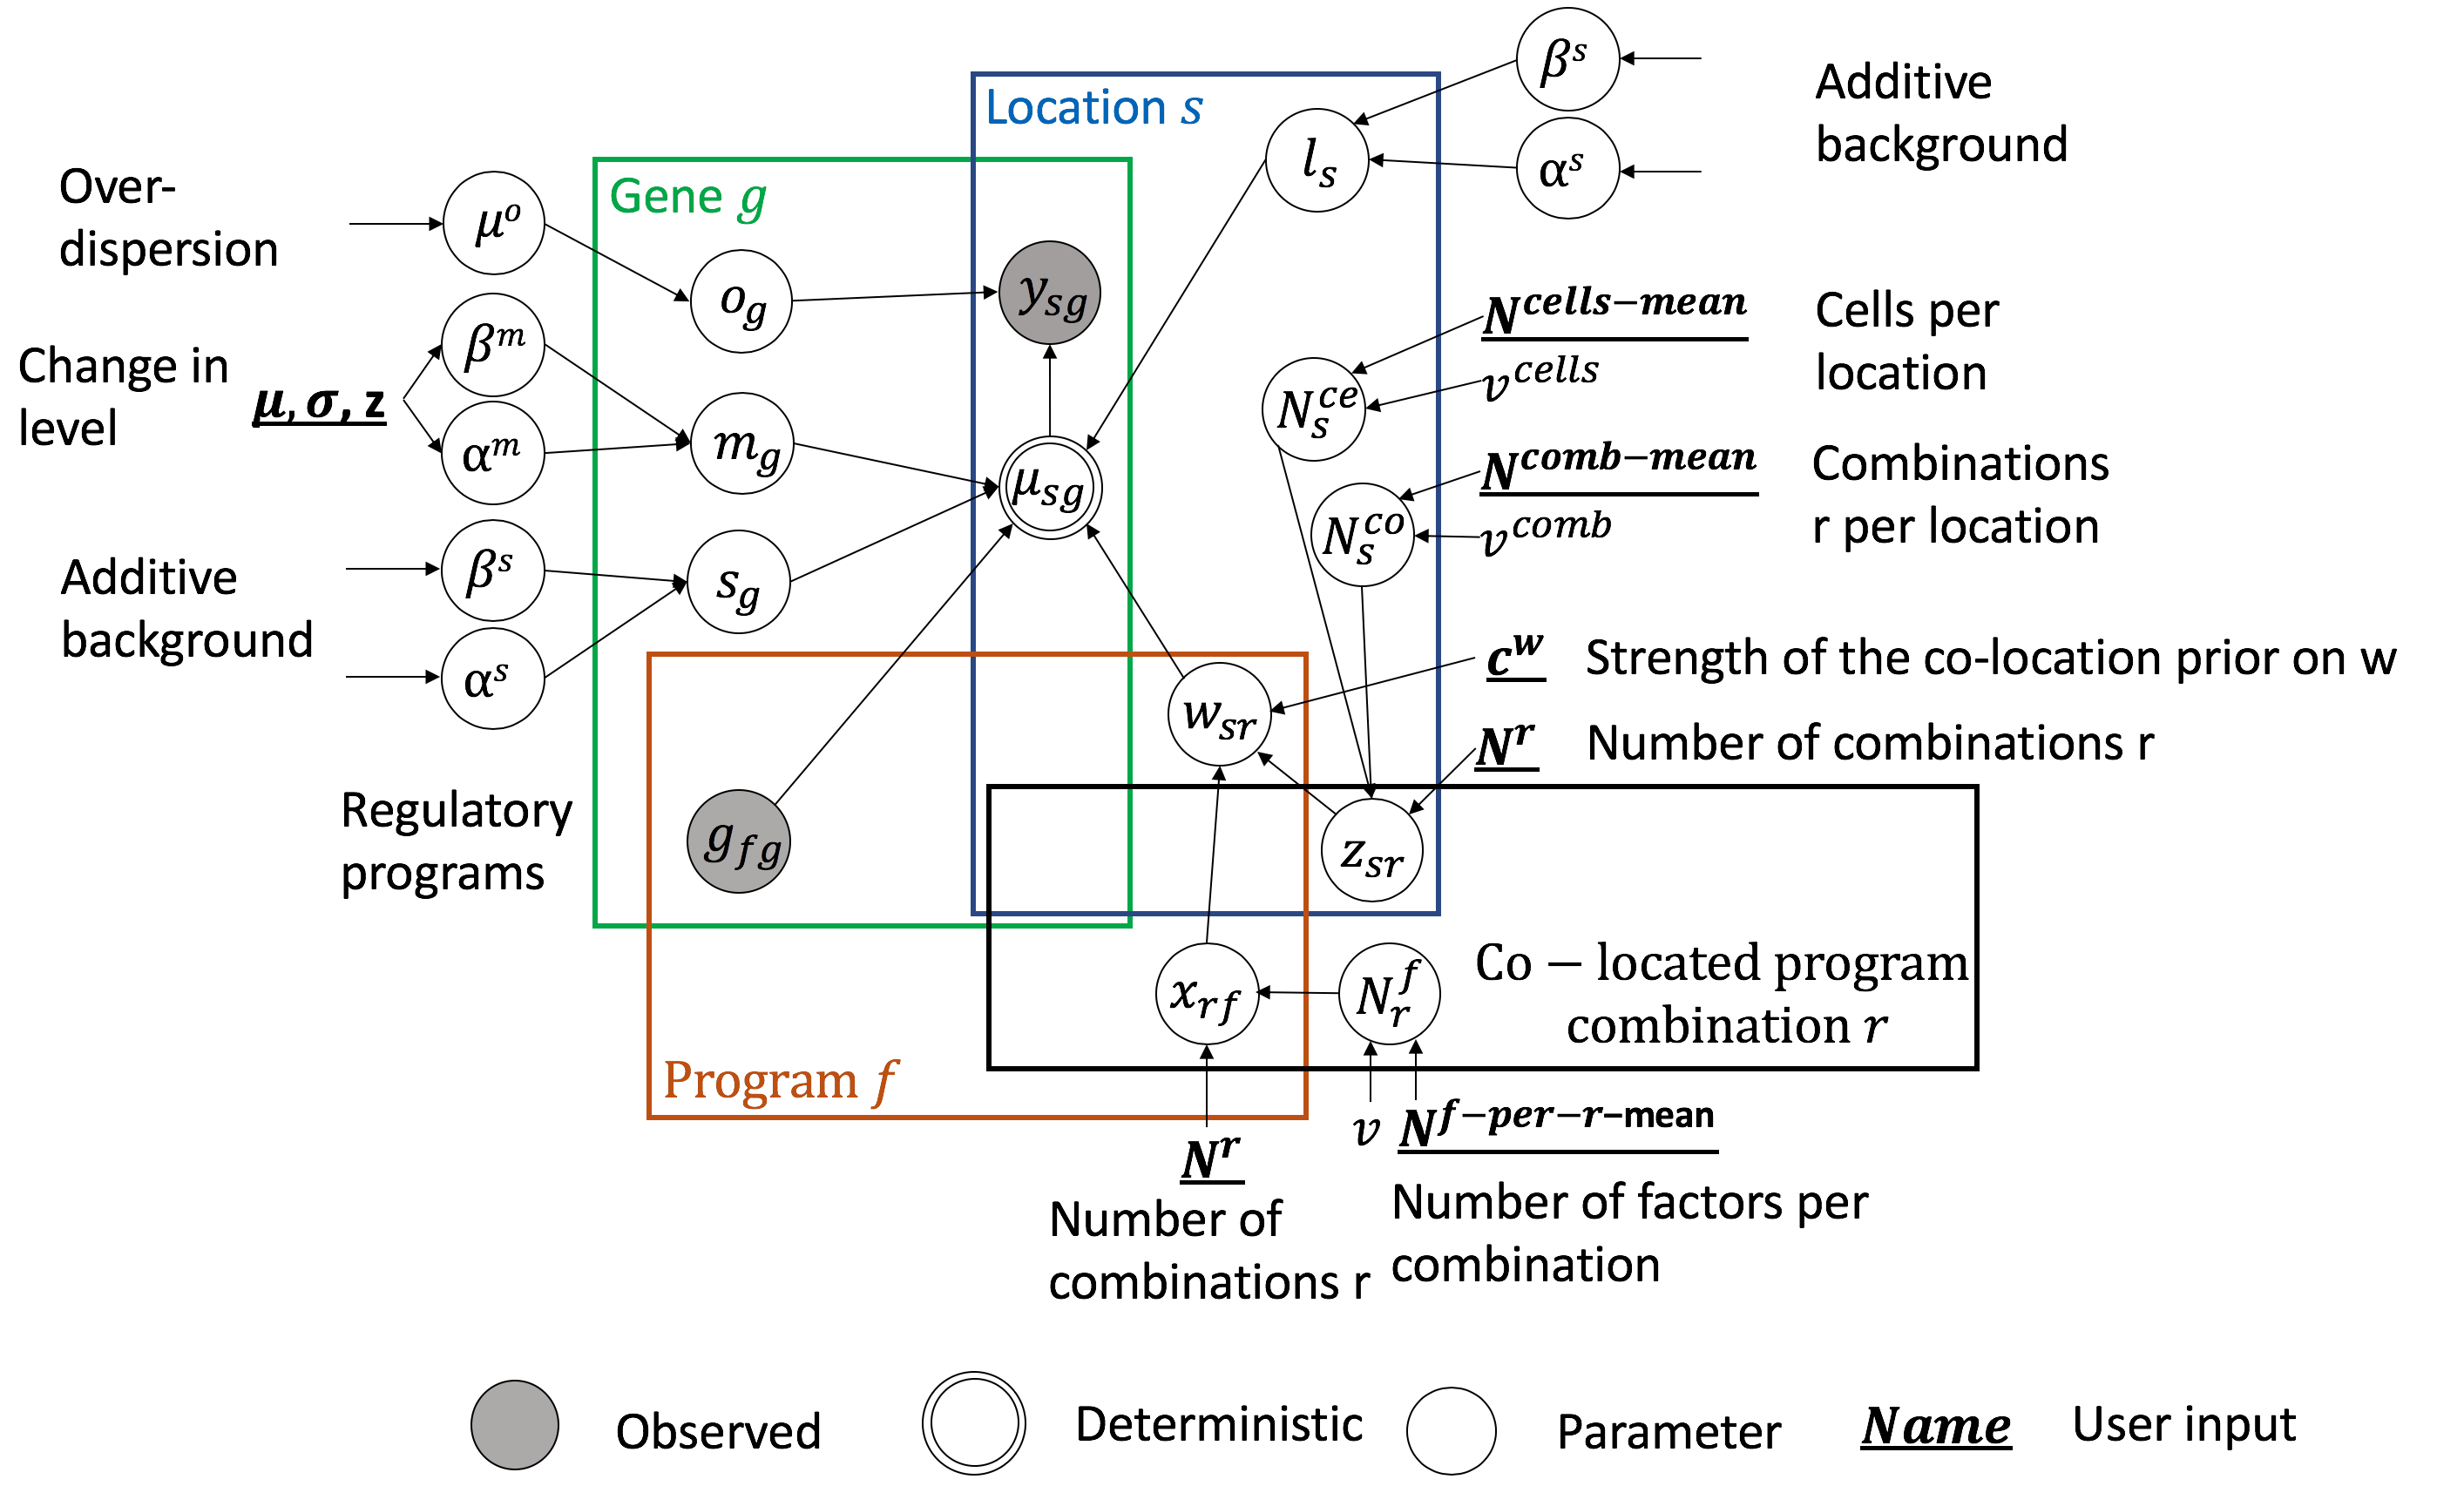
\includegraphics[scale=0.35]{images/CoLocationModelNB4V2.png}
    \caption{Illustration of the corresponding graphical model. \red{Need updating with whatever new names we choose}}
    \label{fig:graphical_model}
\end{figure}

\subsection{Multi-experiment extension of cell2location model} \label{c2l_multi}

When analyzing multiple spatial data sets jointly, where $e=\{1..E\}$ denote individual experiments, such as 10X Visium square capture area and Slide-Seq V2 "puck", the over-dispersion parameter $\alpha_{e,g}$ and additive background parameter $s_{e,g}$ are fit separately for each experiment as well as genes. Specifically, $\alpha_{e,g}$ depends on $o_{e,g}$ which is modelled as independent and exponentially distributed (eq \ref{eq:c2l:21multi} and \ref{eq:c2l:22multi}:
    \begin{equation} \label{eq:c2l:21multi}
    \alpha_{e,g} = 1 / o_{e,g} ^ 2
    \end{equation}
    \begin{equation} \label{eq:c2l:22multi}
    o_{e,g} \sim \mathtt{Exponential}(\mu^o)
    \end{equation}

Individual locations belong to experiments, $s \in e$, therefore the only following parameters are shared between experiments:
\begin{enumerate}

    \item The same reference cell type signatures $g_{f,g}$ are used for all experiments.
    
    \item $m_{g}$, the change in sensitivity between technologies is shared across experiments, improving the ability of the model to distinguish low $m_{g}$ from zero cell abundance $w_{r,f}$. This is equivalent to regressing out the effect of technology but not the effect of individual experiment. 
    
    \item $x_{r,f}$, latent groups $r$ of reference cell types $f$ with similar spatial abundance, and it's hierarchical prior, $N_r^{x}$, the number of cell types per group
    
    \item Variables that serve as hierarchical priors (single value for each variable): $\alpha^m$, $\beta^m$, $\alpha^l$, $\beta^l$, $\alpha^s$, $\beta^s$, $\mu^o$
    
\end{enumerate}

\begin{equation} \label{eq:c2l:1multi}
D_{s,g} \sim \mathtt{NB}(\mu_{s,g}, \alpha_{e,g}) \\
\end{equation}

\red{\< Oli's suggestion (eq 27):}
\begin{equation} \label{eq:c2l:1multiO}
D_{s,g}^{e} \sim \mathtt{NB}(\mu_{s,g}^{e}, \alpha_{g}^{e}) \\
\end{equation}

\subsection{Inference} \label{c2l_inference}

Variational Bayesian Inference is used to approximate the posterior, specifically black-box Automatic Differentiation Variational Inference (ADVI) implemented in pymc3 framework \cite{salvatier_probabilistic_2016}. Appropriately transformed (to positive scale) univatiate normal distributions are used to approximate each parameter. Inference is achieved by maximising log-likehood of the data and minimising KL divergence from the posterior to prior (ELBO loss function). Posterior mean and standard deviation for each parameter where computed using 1000 samples from the Variational posterior distribution.
Several restarts are performed to evaluate the stability of the inferred posterior distribution (usually 2). Under default parameters inference is very stable so no selection of the best model is performed (the first training restart is used). Validity of selected hyper-parameters is evaluated using prior predictive check. Performance of the training is evaluated by performing the posterior predictive check for the accuracy of the model at reconstructing expression levels of each gene $g$ in each location $s$; and by evaluating consistency of inferred $w_{sf}$ parameters between the training restarts.

\subsection{Processing of the spatial expression matrix} \label{c2l_sp_proc}
Expression $D_sg$ counts of each gene $g$ in each location $s$ are obtained from running 10X Spaceranger 1.0.0 on sequencing data from the 10X Visium experiment described in Section \ref{data_analysis_mouse_brain}. Untransformed and unnormalised count matrix was filtered to include genes expressed in the single cell reference $g_fg$ and used as input to the model.

\subsection{Estimation of reference expression signatures of cell types} \label{c2l_ref_prog}

We obtain reference expression signatures of cell types $G$ from scRNA-seq  expression data $J=\{d_{s,g}\}$ of each gene $g=\{1..G\}$ in cell $c=\{1..C\}$. Untransformed and unnormalised count matrix $J_{c,g}$ is filtered to select expressed genes as described in \ref{data_analysis_mouse_brain}. We use following 2 alternative methods to compute $g_{f,g}$:
\begin{enumerate}
    \item Analytically computing single cell reference cluster centroids for each gene $g$ and cell cluster $f=\{1..F\}$. This method is very computationally efficient and gives very good mapping quality (measured on simulated data) when the scRNA-seq reference is a single sample matching the source of spatial data $D_{s,g}$, or a few samples with no strong batch effect between them.
    \item To address the usage of challenging reference data composed of multiple batches $e=\{1..E\}$ and technologies $t=\{1..T\}$ the biological expression of each gene $g$ in each single cell reference cluster $f$ is estimated using a regularised Negative Binomial regression. The model accounts for the global sequencing coverage $h_e$, gene-specific difference in sensitivity between technologies $p_{t,g}$ and background expression $b_{e,g}$ in each sample $e$. It models unexplained variance (overdispersion $\alpha_g$) and count nature of the data using Negative Binomial distribution:
    \begin{equation} \label{eq:c2l_ref_prog:1}
    J_{c,g} \sim \mathtt{NB}(\mu_{c,g}, 1 / \alpha_g^2)
    \end{equation}
    \begin{equation} \label{eq:c2l_ref_prog:2}
    \mu_{c,g} = (g_{f,g} + b_{e,g}) \: {h_e} \: p_{t,g}
    \end{equation}
    All model parameters are constrained to be positive to simplify interpretation. Weak L2 regularisation of $g_{f,g}$ / $b_{e,g}$ / $\alpha_g$ and penalty for large deviations of $h_e$ and $p_{t,g}$ from 1 is used. $g_{f,g}$ is initialised at analytical average for each $f$ and $b_{e,g}$ is initialised at average expression of each gene $g$ in each sample $e$ divided by a factor of 10. The informative initialisation leads to fast convergence.  \newline
    Pytorch implementation of training using mini batches makes the model fast (30sec-5min on GPU) and scalable to very large data sets (>100k cells). Maximum a posteriori optimisation is used to find parameters of this model with batch size of 1024 cells, ADAM optimiser learning rate 0.01. The number of epochs needed for training is determined using cross-validation performed on held-out 10 percent of cells. \newline
    To verify that the model successfully accounted to non-biological sample effects $h_e$, $p_{t,g}$ and $b_{e,g}$ a corrected the expression matrix $J^{corrected}_{c,g}$ is obtained by normalising $J_{c,g}$:
    \begin{equation} \label{eq:c2l_ref_prog:3}
    J^{corrected}_{c,g} = J_{c,g} / ({h_e} \: p_{t,g}) - b_{e,g}
    \end{equation}
    $J^{corrected}_{c,g}$ matrix is subjected to standard scanpy workflow \cite{wolf_scanpy_2018} to verify the mixing of the cells from different samples and technologies within matching cells types (Fig S16A).

\end{enumerate}

\subsection{Differential expression between reference signatures} \label{c2l_ref_prog_diff_expression}

To identify markers of reference cell types we implemented the regression model presented in \ref{c2l_ref_prog} using a principled Bayesian framework. Correspondingly, the model accounts for the global sequencing coverage $h_e$, gene-specific difference in sensitivity between technologies $p_{t,g}$ and background expression $b_{e,g}$ in each sample $e$. It models unexplained variance (overdispersion $\alpha_g$) and count nature of the data using Negative Binomial distribution:
\begin{equation} \label{eq:c2l_ref_prog_diff:1}
J_{c,g} \sim \mathtt{NB}(\mu_{c,g}, 1 / \alpha_g^2)
\end{equation}
\begin{equation} \label{eq:c2l_ref_prog_diff:2}
\mu_{c,g} = (g_{f,g} + b_{e,g}) \: {h_e} \: p_{t,g}
\end{equation}

All model parameters are constrained to be positive to simplify interpretation. The following priors are used with empirically chosen hyper-parameters:
\begin{equation} \label{eq:c2l_ref_prog_diff:3}
g_{f,g} \sim \mathtt{Gamma}(gs, gr)
\end{equation}
\begin{equation} \label{eq:c2l_ref_prog_diff:4}
gs \sim \mathtt{Gamma}(mu=0.3, var=mu/3)
\end{equation}
\begin{equation} \label{eq:c2l_ref_prog_diff:4}
gr \sim \mathtt{Gamma}(mu=0.8, var=mu/3)
\end{equation}

\begin{equation} \label{eq:c2l_ref_prog_diff:5}
b_{eg} \sim \sim \mathtt{Gamma}(bs, br)
\end{equation}
\begin{equation} \label{eq:c2l_ref_prog_diff:6}
bs \sim \mathtt{Gamma}(mu=0.45, var=mu/3)
\end{equation}
\begin{equation} \label{eq:c2l_ref_prog_diff:7}
br \sim \mathtt{Gamma}(mu=11, var=mu/3)
\end{equation}

\begin{equation} \label{eq:c2l_ref_prog_diff:8}
h_e \sim \mathtt{Gamma}(6, 6)
\end{equation}
\begin{equation} \label{eq:c2l_ref_prog_diff:9}
p_{tg} \sim \mathtt{Gamma}(10, 10)
\end{equation}

Similarly, to the maximum likelihood model, $g_{f,g}$ is initialised at analytical average for each $f$ and $b_{e,g}$ is initialised at average expression of each gene $g$ in each sample $e$ divided by a factor of 10.  \newline
Pyro implementation of training using mini batches makes model comparably scalable and fast. Optimisation is used to find Variational Posterior of the parameters with batch size of 1024 cells, ADAM optimiser learning rate 0.001. The training is stopped before $p(J_{c,g} | \mu_{c,g}, 1 / \alpha_g^2$) starts decreasing. Posterior mean and standard deviation for each parameter where computed using 1000 samples from the Variational posterior distribution. \newline

To identify genes most specific to each reference cell type $f$, such as astrocyte subtypes, the following algorithm was applied to the posterior of $g_{f,g}$:
\begin{enumerate}
    \item Normalise each sample from the posterior distribution such that $g^{norm}_{f,g} = g_{f,g} / \sum_{g} g_{f,g}$.
    \item Compute 5\% quantile of the posterior distribution of $g^{norm}_{f,g}$ to incorporate uncertainty in the estimates
    \item Rank genes for each cell type $f$ using 5\% quantiles of normalised expression $g^{norm}_{f,g}$
\end{enumerate}


\subsection{Nuclei Segmentation} \label{c2l_segmentation}

To perform nuclei segmentation, H&E-stained image of the Visium-profiled tissue was used. The image was acquired using Hamamatsu slide scanner as described in the section on experimental processing. Full resolution images were divided into smaller parts of size about 1000 by 1000 pixels. Then a state-of-the-art convolutional neural network (CNN)-based segmentation pipeline described in \cite{caicedo_nucleus_2019} was used and available at \cite{'https://github.com/selimsef/dsb2018_topcoders'}. An ensemble of 32 pre-trained CNNs each with Unet- or FPN-like architecture was used to classify pixels to 3 classes: background, nuclei and nuclei boundaries. Predicted segmentation masks were averaged across CNNs, then a watershed algorithm was applied to refine predicted boundaries and separate individual nuclei. As a final step, a gradient boosting model over morphological features such as nuclei colour, shape and size was used to remove false-positively detected nuclei.  
Obtained individual nuclei masks were used to compute several morphological features such as area (count of pixels in a mask), shape (ratio of lengths of the major and minor axis of an ellipse fitted to the mask) and position (center of mass of the image containing individual mask).
Kd-tree approach was used to assign nuclei locations to Visium spots efficiently. Kd-tree implementation from the scikit-learn package was used.


\section{Identifying tissue regions by clustering} \label{auto_clustering}

The cell density $w_{sf}$ (eq. \ref{eq:c2l:4}) inferred by cell2location model serves as a proxy to cell density. This enables describing similarity of locations (spots) by constructing a KNN graph that represents connectivity of locations in terms of their in cell composition (N neighbours = 20 for human lymph node, 38 for the mouse brain). Standard implementation of Leiden clustering (function scanpy.tl.leiden) in the scanpy package \cite{wolf_scanpy_2018} can utilise cell composition KNN graph to characterise organisation of the tissue. We performed Leiden clustering with default arguments (resolution ?? for human lymph node, resolution ?? for the mouse brain). Obtained regions were cross-referenced with the mouse brain anatomy using corresponding histology images and similar clusters were merged to generate the broad region map.

\section{Combinations of co-located cell types} \label{cell_neighbourhoods}

To map out cellular compartment of the tissue we co-opted non-negative matrix factorisation model (NMF). Absolute cell type abundance $w_{sf}$ of each cell type $f$ across locations $s$ is modelled as an additive function of the cell type groups (cellular compartments) $r$. This means that several cellular compartments can be present in one location (Fig S16B). Cell type abundance is therefore a function of the following non-negative components:  
\begin{equation} \label{eq:circ:1}
w_{s,f} = (\sum_{r} {i_{s,r} \: k_{r,f} \: m_{f}})
\end{equation}

\begin{enumerate}
    \item $k_{r,f}$ represents the proportion of cells of each type (reference signatures) $f$ that correspond to each cell type group $r$, normalised for total abundance of each cell type $m_{f}$.
    \item $m_{f}$ cell type budget accounts for the difference in abundance between cell types.
    \item $i_{sr}$ is proportional to the number of cells from each neighbourhood $r$ in each location $s$, and shows the abundance of cell types groups $r$ in locations $s$.
\end{enumerate}

In practice $q_{rf} = k_{rf} \: m_{f}$ is obtained from scikit-learn NMF and normalised by the sum across combinations $r$ to obtain $k_{rf}$:
\begin{equation} \label{eq:circ:2}
k_{rf} = q_{rf} / (\sum_{r} q_{rf})
\end{equation}

Inference is performed using standard NMF in the scikit-learn package \cite{scikit-learn}. The model is trained multiple times to evaluate stability of the identified cellular compartments. The first training iteration is selected. 

We hypothesise that linear dependencies in the abundance of cell types across locations reflects the interaction between these cell types, specifically, any interaction that could affect mutual location of these cell types. For this reason we tested this approach on human lymph nodes, a tissue where locations of cell types are determined by their interactions. 10X Visium technology combines cell types located within the $55\mu m$ diameter of capture areas, a distance at which local paracrine signals and direct adhesive contacts can act, likely driving linear dependencies in cell abundance. We assume that the signal does not propagate between neighbouring locations spaced by $45\mu m$ gaps, therefore using proximity information is not essential. Therefore we note that that this interpretation of NMF decomposition of cell abundances is a unique feature of technologies that aggregate multiple cells within single locations which does not directly apply to technologies with increased resolution (Slide-Seq V2).

Potential cell interactions driving linear dependencies in cell type abundance can be classified into:
\begin{itemize}
    \item Signals promoting proliferation and survival of other cell type
    \item Adhesion molecules that increase the frequency of contacts 
    \item Recruitment signals such as CXCR5 / CXCL13 \cite{van_de_pavert_chemokine_2009}
    \item Repulsive signals, inhibiting the action of chemotaxis signals such as PD-1 / PD-L1 interactions \cite{shi_pd-1_2018}
    \item Interactions that induce new transcriptional states 
\end{itemize}

\printbibliography

\end{document}